\chapter{Architettura del sistema}
\label{cap:architettura}

Il sistema è organizzato come una pipeline distribuita su due microcontrollori indipendenti che comunicano via UART. Una terza unità, il PC host, ha il ruolo di sorgente delle immagini e di destinazione del risultato finale. Questo capitolo descrive la suddivisione dei compiti tra i tre nodi, la disposizione fisica dei collegamenti e le motivazioni che hanno guidato la scelta di un'architettura distribuita.

\section{Suddivisione dei compiti}
\label{sec:suddivisione}

Il flusso di elaborazione attraversa tre nodi in sequenza, ognuno responsabile di una fase specifica della pipeline ALPR:

\begin{itemize}
    \item Il \textbf{PC host} esegue lo script Python di test, che si occupa del pre-processing dell'immagine (conversione in scala di grigi e ridimensionamento a $192\times192$~pixel), dell'invio del payload al sistema embedded via UART e della visualizzazione del risultato finale. Il PC non partecipa all'inferenza.
    \item La \textbf{Board A} riceve l'immagine grayscale, ne calcola la quantizzazione INT8, esegue la rete YOLOv8-tiny per individuare la targa, applica la \textit{Non-Maximum Suppression} e ritaglia la porzione di immagine corrispondente. Questo viene quindi ridimensionato a $128\times64$~pixel tramite interpolazione \textit{nearest-neighbor}. Il crop così ottenuto viene inoltrato alla Board B e ne attende la risposta che viene successivamente mandata al PC.
    \item La \textbf{Board B} riceve il ritaglio in scala di grigi $128\times64$~pixel, lo espande sui tre canali RGB attesi dalla rete OCR, esegue il modello CCT-XS, decodifica la sequenza di logit in una stringa alfanumerica e la restituisce alla Board A.
\end{itemize}

La Figura~\ref{fig:flusso_nodi} riassume il flusso di dati e l'evoluzione del payload lungo la pipeline.

\begin{figure}[H]
    \centering
    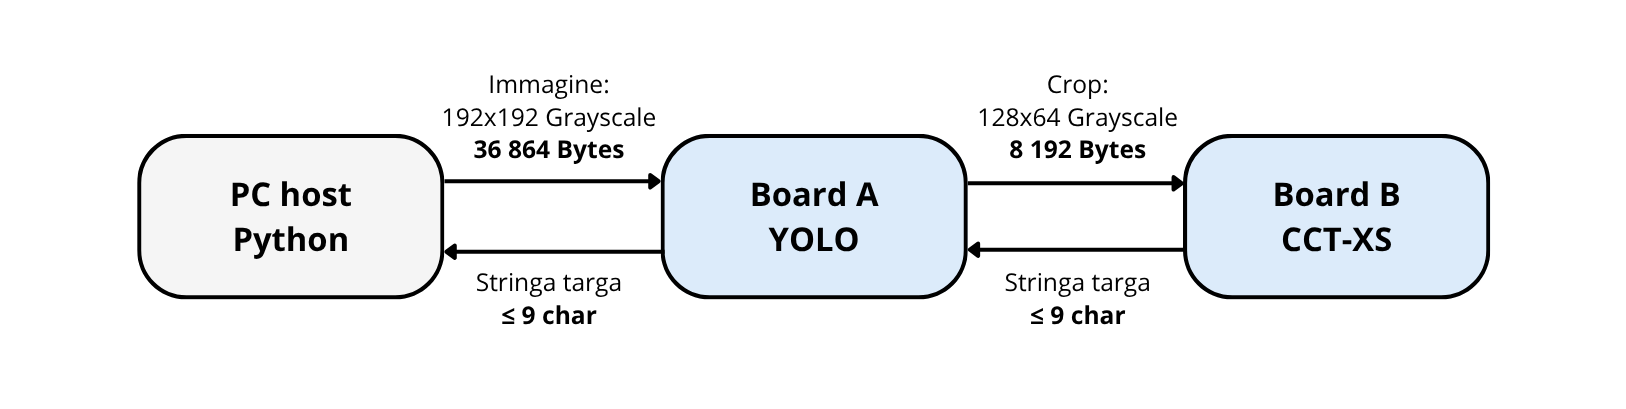
\includegraphics[width=1.1\textwidth]{images/flusso_nodi.png}
    \caption{Flusso dei dati tra i nodi lungo la pipeline}
    \label{fig:flusso_nodi}
\end{figure}

\newpage

\iffalse
\section{Motivazioni dell'architettura distribuita}
\label{sec:motivazioni}

La scelta di distribuire la pipeline su due microcontrollori, anziché eseguire entrambi i modelli su un singolo dispositivo, deriva da un vincolo concreto di memoria. Una stima preliminare ha mostrato che la sola rete YOLO occupa oltre 400~KB di RAM per le \textit{activation}, mentre la rete CCT-XS ne richiede circa 290~KB. La somma supera la capacità della SRAM principale della STM32H745, che è di 512~KB. Eseguire i due modelli sulla stessa unità avrebbe richiesto un meccanismo di scambio dei pesi tra Flash e RAM tra una fase e l'altra, oppure un'allocazione manuale su regioni di memoria diverse, con conseguente complessità implementativa e perdita di prestazioni.

Distribuire i due modelli su schede separate elimina questo problema alla radice: ciascuna scheda ospita un solo modello, dispone della totalità della propria SRAM per le activation e può essere programmata in modo indipendente. Il prezzo da pagare è la necessità di trasferire i dati tra le due schede attraverso un canale di comunicazione, scelta che però introduce contemporaneamente un caso d'uso didatticamente interessante --- la sincronizzazione tra microcontrollori --- coerente con gli obiettivi del corso di Sistemi Operativi Dedicati.
\fi

\section{Collegamenti hardware}
\label{sec:collegamenti}

Le due schede sono collegate al PC host e tra loro attraverso tre canali UART seriali, tutti operanti a 115\,200~baud con configurazione 8N1. La Figura~\ref{fig:schema_collegamenti} mostra lo schema fisico dei collegamenti tra le due schede STM, evidenziando le porte coinvolte e i pin del microcontrollore utilizzati per la comunicazione tra le board che è stata realizzata tramite l'interfaccia \textbf{USART2} collegando fisicamente i pin in modalità incrociata: il pin \textbf{PD5 (TX)} di ciascuna scheda è connesso al pin \textbf{PD6 (RX)} dell'altra, in modo che la trasmissione di una corrisponda alla ricezione dell'altra. È necessario inoltre collegare tra loro i pin \textbf{GND} delle due schede, in modo da stabilire un riferimento di tensione comune: poiché la comunicazione seriale UART è single-ended, il livello logico del segnale TX viene interpretato dalla scheda ricevente rispetto al proprio ground, e in assenza di una massa condivisa i livelli di tensione risulterebbero indefiniti, rendendo la comunicazione inaffidabile o del tutto impossibile.\\ 
Lato firmware, l'interfaccia è stata abilitata e configurata tramite il sistema di \textit{Device Tree overlay} di Zephyr RTOS, come visibile nel Listato \ref{lst:abilitazione_pin}. Questo approccio consente di separare nettamente la configurazione hardware dal codice applicativo, delegando al Device Tree la gestione dei mapping dei pin e dei parametri del bus.\\
\begin{lstlisting}[style=stileYAML, caption={Device Tree overlay per l'abilitazione dei pin PD5 e PD6}, label={lst:abilitazione_pin}]
&usart2 {
    status = "okay";
    current-speed = <115200>;
    pinctrl-0 = <&usart2_tx_pd5 &usart2_rx_pd6>;
    pinctrl-names = "default";
};
\end{lstlisting}
\begin{figure}[H]
    \centering
    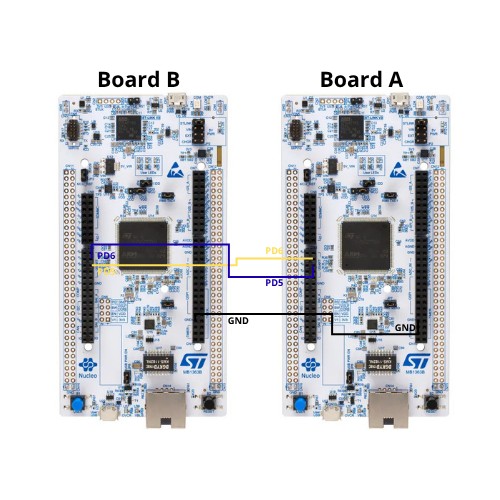
\includegraphics[width=0.55\textwidth]{images/immagine_collegamenti.png}
    \caption{Schema dei collegamenti tra le due Board}
    \label{fig:schema_collegamenti}
\end{figure}

Il collegamento tra il PC e la Board A sfrutta l'interfaccia \textbf{ST-Link} integrata sulla scheda Nucleo, che espone automaticamente un canale UART virtuale mappato sulla USART3 del microcontrollore. In questo modo il PC può inviare l'immagine da elaborare e ricevere il risultato del riconoscimento tramite una semplice comunicazione seriale, senza che il firmware debba gestire alcuno stack USB dedicato: la Board A interagisce con l'host esattamente come farebbe con qualsiasi altro dispositivo seriale. La Board B, invece, non dovendo comunicare direttamente con il PC, richiede unicamente l'alimentazione tramite cavo USB per essere operativa all'interno del sistema.\\
La Figura \ref{fig:setup} illustra il banco di prova allestito per la validazione del sistema, con evidenza dei collegamenti fisici realizzati tra le due schede e il PC.

\begin{figure}[H]
    \centering
    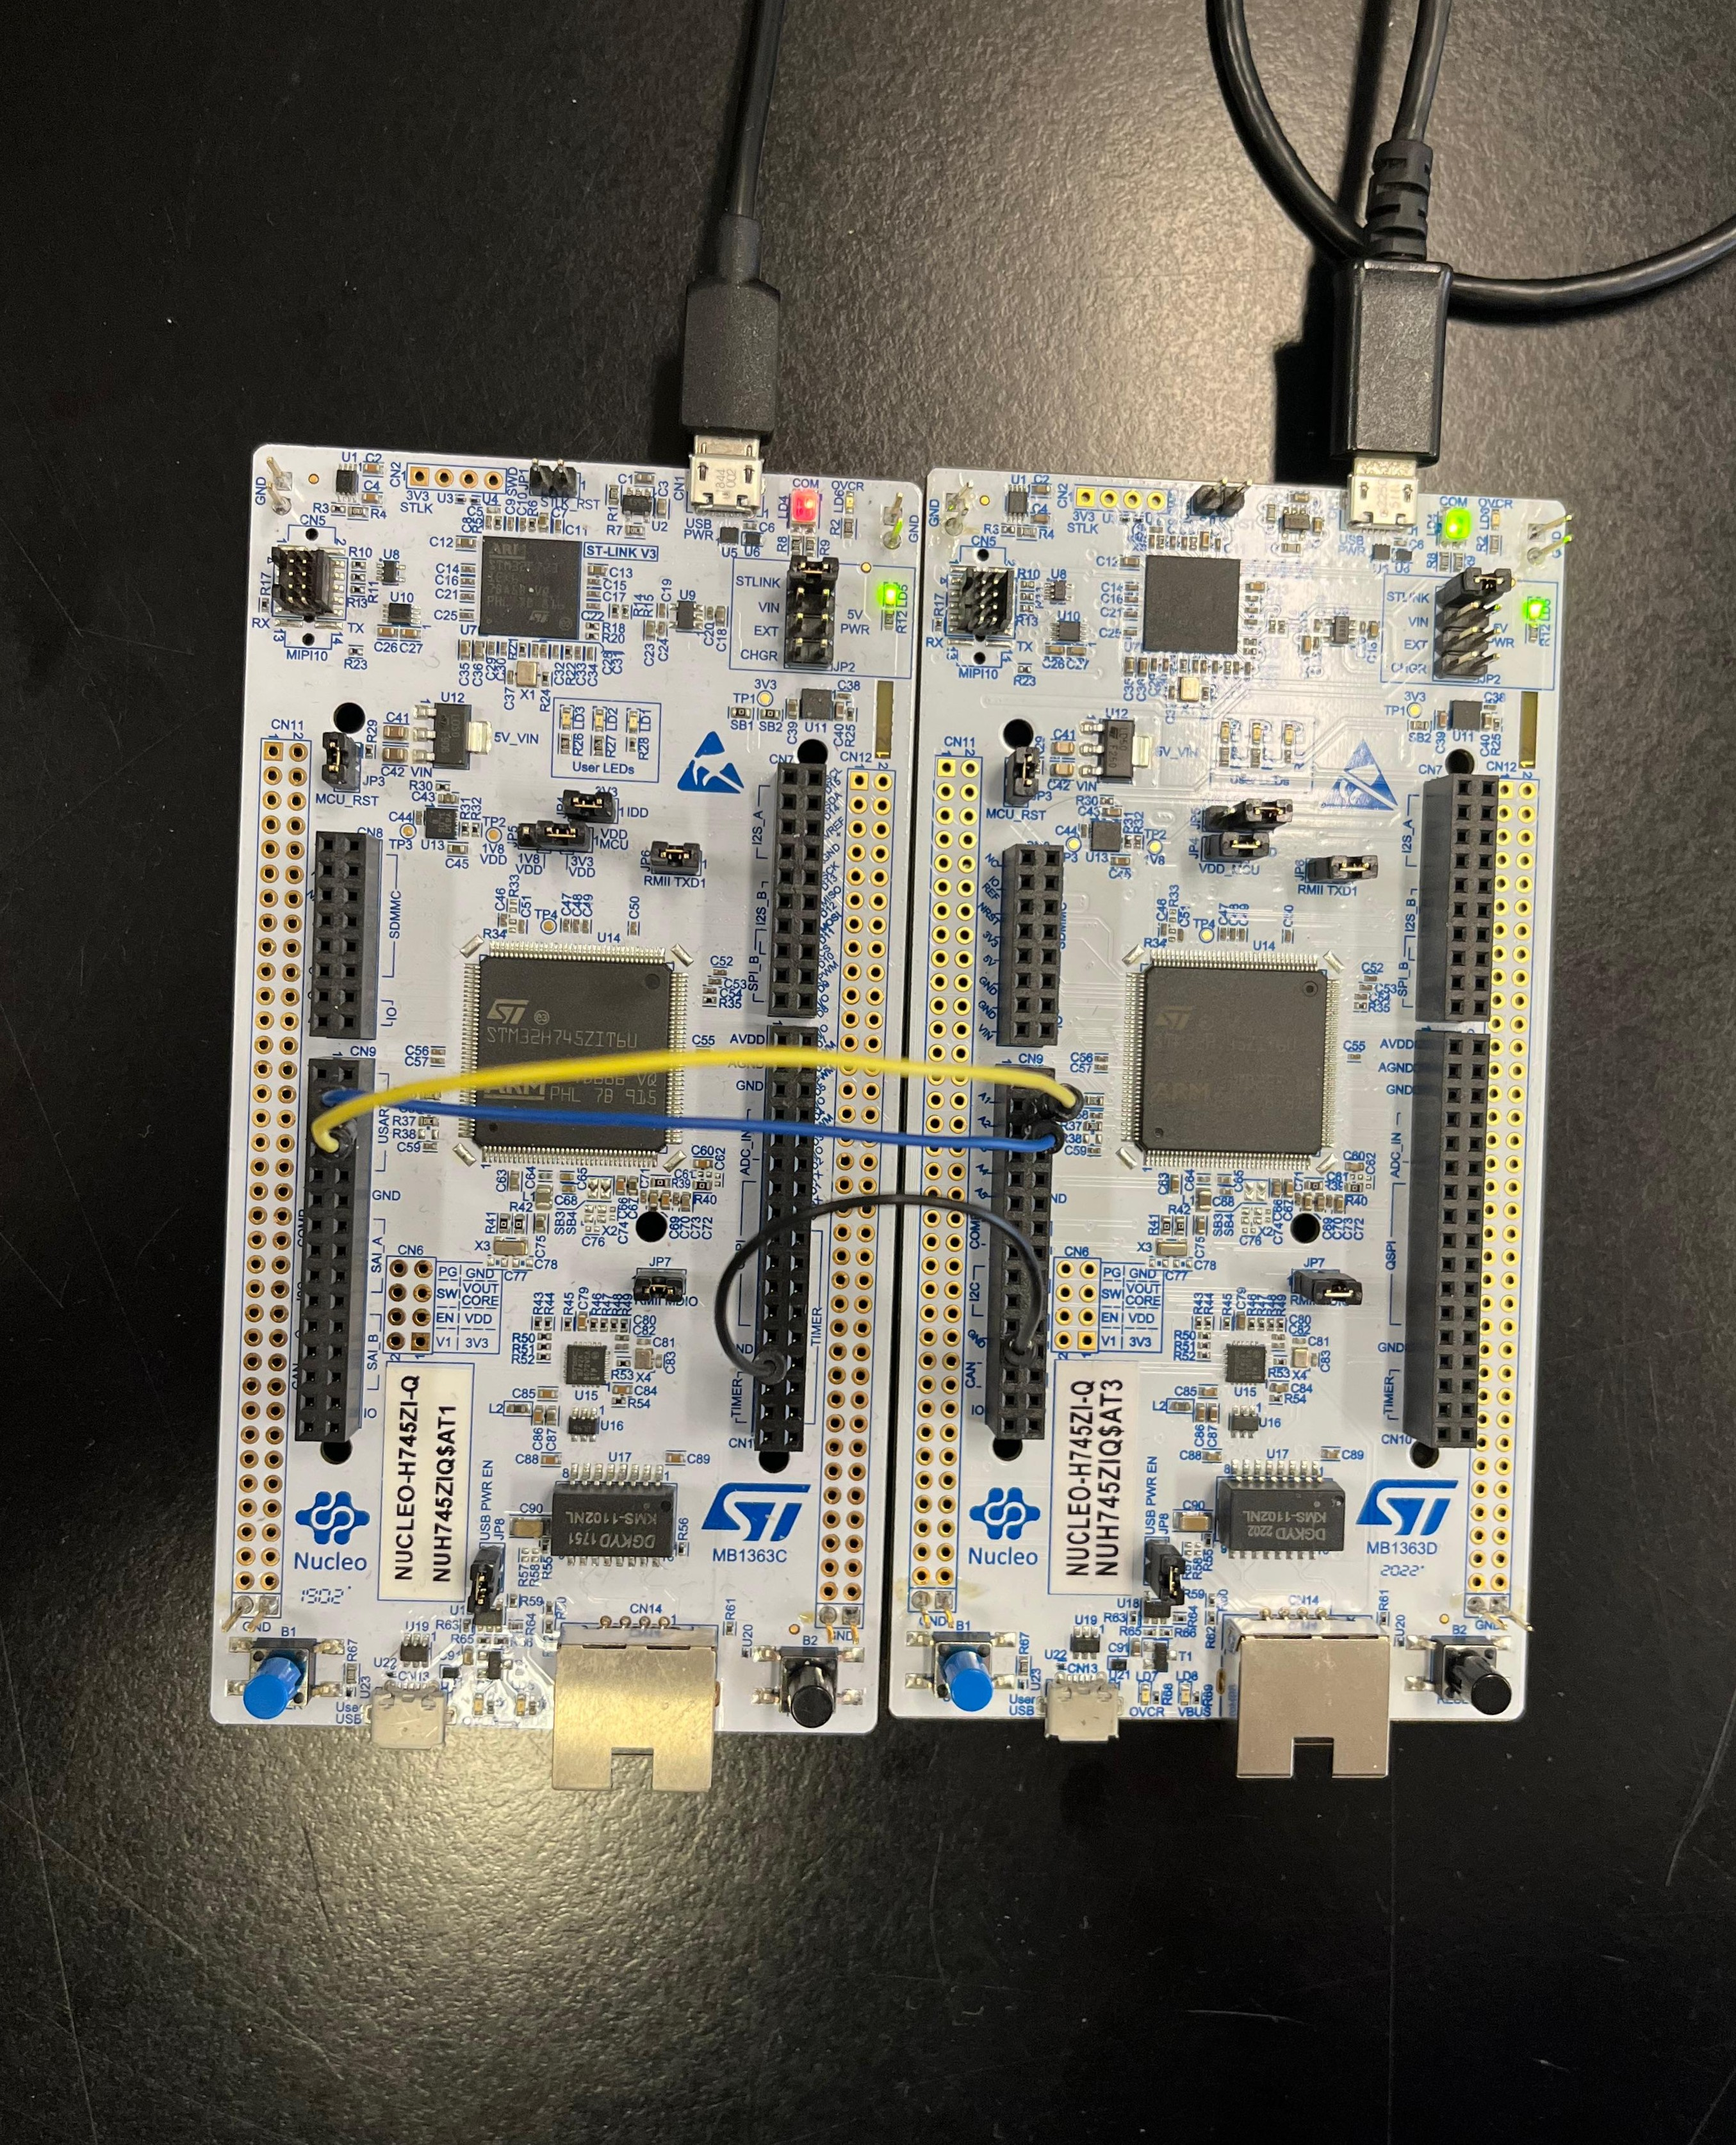
\includegraphics[width=0.7\textwidth]{images/setup_board.jpeg}
    \caption{Fotografia del banco di prova con le due schede collegate}
    \label{fig:setup}
\end{figure}

